\documentclass[plain,worksheet,]{inVerba-notes}
\begin{document}
\begin{center}
    \Large \textbf{Sensory and Motor Systems --- Problem Set 1}
\end{center}
\medskip
\begin{enumerate}
    \item Define equilibrium for an ion (within the context of the neuronal membrane). Your answer should mention forces.
    
    
    \vspace{80pt}
    
    \item What is the membrane potential at steady state in a cell with a membrane that is only permeable to calcium (Calcium out = 1.9mM, Calcium in= 0.0002mM)? 
    
    \vspace{80pt}

    \item If Vm is -70mV and external sodium is 145mM and internal is 10 mM. Calculate the driving force for sodium ions after Nav channels open.
    
    \vspace{120pt}

    \item Please explain the shape of the current voltage relationship for both voltage gated sodium and potassium ion channels.
\end{enumerate}
    \bigskip
    
    \begin{center}
        

\tikzset{every picture/.style={line width=0.75pt}} %set default line width to 0.75pt        

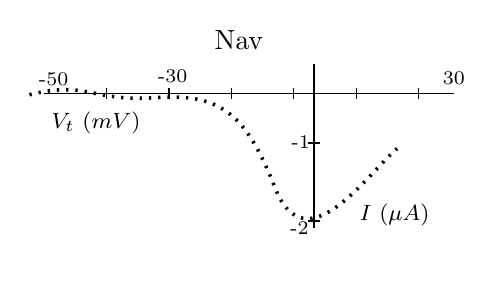
\begin{tikzpicture}[x=0.75pt,y=0.75pt,yscale=-0.7,xscale=0.7]
%uncomment if require: \path (0,300); %set diagram left start at 0, and has height of 300

%Straight Lines [id:da30256639311913547] 
\draw    (183.6,160) -- (465.5,160) (226.6,156) -- (226.6,164)(269.6,156) -- (269.6,164)(312.6,156) -- (312.6,164)(355.6,156) -- (355.6,164)(398.6,156) -- (398.6,164)(441.6,156) -- (441.6,164) ;
%Straight Lines [id:da24911735771459287] 
\draw [line width=0.75]    (369.6,139.8) -- (369.6,252.8) (373.6,193.8) -- (365.6,193.8)(373.6,247.8) -- (365.6,247.8) ;
%Curve Lines [id:da6912957926978247] 
\draw  [dash pattern={on 0.84pt off 2.51pt}] [line width=1.3] (173.6,160.8) .. controls (213.6,150.8) and (216.6,165.8) .. (259.6,162.8) .. controls (302.6,159.8) and (321.6,170.8) .. (342.6,224.8) .. controls (363.6,278.8) and (406.6,214.8) .. (426.6,197.8) ;

% Text Node
\draw (456.25,143.1) node [anchor=north west][inner sep=0.75pt]  [font=\small] [align=left] {{\scriptsize 30}};
% Text Node
\draw (360.23,193.3) node  [font=\small] [align=left] {{\scriptsize -1}};
% Text Node
\draw (367.6,252.8) node [anchor=east] [inner sep=0.75pt]  [font=\small] [align=left] {{\scriptsize -2}};
% Text Node
\draw (260.25,142.1) node [anchor=north west][inner sep=0.75pt]  [font=\small] [align=left] {{\scriptsize -30}};
% Text Node
\draw (178.25,144.1) node [anchor=north west][inner sep=0.75pt]  [font=\small] [align=left] {{\scriptsize -50}};
% Text Node
\draw (399,234) node [anchor=north west][inner sep=0.75pt]  [font=\footnotesize] [align=left] {$\displaystyle I\ ( \mu A)$};
% Text Node
\draw (187,171) node [anchor=north west][inner sep=0.75pt]  [font=\footnotesize] [align=left] {$\displaystyle V_{t} \ ( mV)$};
% Text Node
\draw (299.2,115) node [anchor=north west][inner sep=0.75pt]   [align=left] {Nav};


\end{tikzpicture}

    \end{center}

    Explanation:
    \vspace{80pt}
     
    \begin{center}
    

\tikzset{every picture/.style={line width=0.75pt}} %set default line width to 0.75pt        

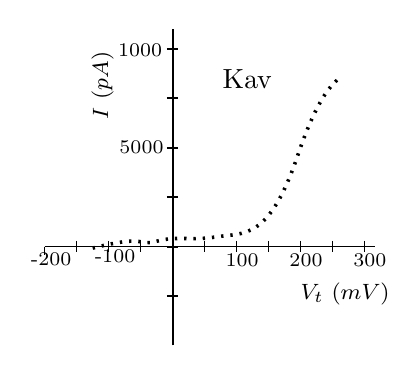
\begin{tikzpicture}[x=0.75pt,y=0.75pt,yscale=-0.7,xscale=0.7]
%uncomment if require: \path (0,300); %set diagram left start at 0, and has height of 300

%Straight Lines [id:da30256639311913547] 
\draw    (281.6,160.8) -- (496.6,160.8) -- (508.6,160.8) (303.6,156.8) -- (303.6,164.8)(325.6,156.8) -- (325.6,164.8)(347.6,156.8) -- (347.6,164.8)(369.6,156.8) -- (369.6,164.8)(391.6,156.8) -- (391.6,164.8)(413.6,156.8) -- (413.6,164.8)(435.6,156.8) -- (435.6,164.8)(457.6,156.8) -- (457.6,164.8)(479.6,156.8) -- (479.6,164.8)(501.6,156.8) -- (501.6,164.8) ;
%Straight Lines [id:da24911735771459287] 
\draw [line width=0.75]    (369.6,228.8) -- (369.6,10.8) (365.6,194.8) -- (373.6,194.8)(365.6,160.8) -- (373.6,160.8)(365.6,126.8) -- (373.6,126.8)(365.6,92.8) -- (373.6,92.8)(365.6,58.8) -- (373.6,58.8)(365.6,24.8) -- (373.6,24.8) ;
%Curve Lines [id:da6912957926978247] 
\draw  [dash pattern={on 0.84pt off 2.51pt}] [line width=1.3] (314.6,161.8) .. controls (354.6,151.8) and (343.72,161.07) .. (358.72,157.07) .. controls (373.72,153.07) and (380.72,157.07) .. (399.72,154.07) .. controls (418.72,151.07) and (435.72,157.07) .. (455.72,98.07) .. controls (475.72,39.07) and (487.72,49.07) .. (482.72,42.07) ;
%Straight Lines [id:da8823789696191159] 
\draw    (281.6,160.8) -- (281.6,166.8) ;

% Text Node
\draw (404.25,164.1) node [anchor=north west][inner sep=0.75pt]  [font=\scriptsize] [align=left] {100};
% Text Node
\draw (364.23,25.3) node [anchor=east] [inner sep=0.75pt]  [font=\scriptsize] [align=left] {1000};
% Text Node
\draw (314.25,161.1) node [anchor=north west][inner sep=0.75pt]  [font=\small] [align=left] {{\scriptsize -100}};
% Text Node
\draw (270.25,163.1) node [anchor=north west][inner sep=0.75pt]  [font=\small] [align=left] {{\scriptsize -200}};
% Text Node
\draw (312,75) node [anchor=north west][inner sep=0.75pt]  [font=\footnotesize,rotate=-270] [align=left] {$\displaystyle I\ ( pA)$};
% Text Node
\draw (456,184) node [anchor=north west][inner sep=0.75pt]  [font=\footnotesize] [align=left] {$\displaystyle V_{t} \ ( mV)$};
% Text Node
\draw (402.2,37) node [anchor=north west][inner sep=0.75pt]   [align=left] {Kav};
% Text Node
\draw (365.23,92.3) node [anchor=east] [inner sep=0.75pt]  [font=\scriptsize] [align=left] {5000};
% Text Node
\draw (448.25,164.1) node [anchor=north west][inner sep=0.75pt]  [font=\scriptsize] [align=left] {200};
% Text Node
\draw (492.25,164.1) node [anchor=north west][inner sep=0.75pt]  [font=\scriptsize] [align=left] {300};


\end{tikzpicture}

    \end{center}

    Explanation:
    \vspace{120pt}


\begin{enumerate}[resume]
    \item Neurons A and B are able to fire at different frequencies. Neuron A’s maximum firing rate is shown below at left; Neuron B’s maximum firing rate is shown at right. Note that in both cases, the vertical lines represent spikes, or individual action potentials. Suggest one specific difference in Na+ or K+ channel properties between these 2 neurons that could explain the different firing rates. Be as specific as you can.
    
    \begin{center}
        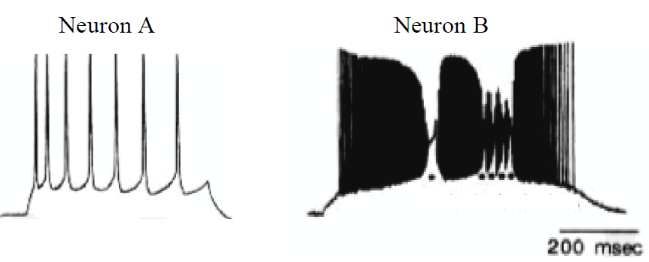
\includegraphics[scale=0.4]{graphs/firing-rate.png}
    \end{center}
    Explanation:
    \vspace{80pt}

    \newpage
    \item Imagine that a mutation causes faster inactivation of sodium channels compared to those that help produced the APs bellow. Draw and explain how the AP shape would change.

    \bigskip
    \medskip
    \begin{center}
        

\tikzset{every picture/.style={line width=0.75pt}} %set default line width to 0.75pt        

\begin{tikzpicture}[x=0.75pt,y=0.75pt,yscale=-1,xscale=1]
%uncomment if require: \path (0,300); %set diagram left start at 0, and has height of 300

%Straight Lines [id:da03816601764574801] 
\draw    (200,210) -- (380,210) ;
%Straight Lines [id:da09549254106437632] 
\draw    (200,210) -- (200,70) ;
%Straight Lines [id:da5948793250120007] 
\draw  [dash pattern={on 0.84pt off 2.51pt}]  (200,180) -- (380,180) ;
%Straight Lines [id:da7466924752229203] 
\draw  [dash pattern={on 0.84pt off 2.51pt}]  (200,80) -- (380,80) ;
%Straight Lines [id:da20607480985401894] 
\draw  [dash pattern={on 0.84pt off 2.51pt}]  (200,200) -- (380,200) ;
%Curve Lines [id:da932064900573946] 
\draw    (200,180) .. controls (215.72,180.07) and (199.28,180.93) .. (230,180) .. controls (260.72,179.07) and (255,79) .. (266.72,79.07) .. controls (278.43,79.13) and (275.28,205.93) .. (310,200) .. controls (344.72,194.07) and (341.72,177.07) .. (380,180) ;

% Text Node
\draw (281,216) node [anchor=north west][inner sep=0.75pt]  [font=\scriptsize] [align=left] {time};
% Text Node
\draw (185,147) node [anchor=north west][inner sep=0.75pt]  [font=\scriptsize,rotate=-270] [align=left] {mV};


\end{tikzpicture}

    \end{center}
    Explanation:
    \vspace{120pt}
\end{enumerate}    
\begin{enumerate}[resume]
    \item When a normal, healthy squid axon is voltage-clamped in artificial seawater, one obtains the following current (I) record in response to a step change in \si{V_m} from \SI{-70}{mV} to \SI{+20}{mV}.
    
    \bigskip
    \bigskip
    \begin{center}
        

\tikzset{every picture/.style={line width=0.75pt}} %set default line width to 0.75pt        

\begin{tikzpicture}[x=0.75pt,y=0.75pt,yscale=-1,xscale=1]
%uncomment if require: \path (0,263); %set diagram left start at 0, and has height of 263

%Straight Lines [id:da16011518847864004] 
\draw    (169.6,199) -- (450.6,199) (195.6,195) -- (195.6,203)(221.6,195) -- (221.6,203)(247.6,195) -- (247.6,203)(273.6,195) -- (273.6,203)(299.6,195) -- (299.6,203)(325.6,195) -- (325.6,203)(351.6,195) -- (351.6,203)(377.6,195) -- (377.6,203)(403.6,195) -- (403.6,203)(429.6,195) -- (429.6,203) ;
%Straight Lines [id:da6331484236419908] 
\draw    (169.6,199) -- (169.6,209.8) ;
%Straight Lines [id:da9468556493718451] 
\draw    (450.6,198.8) -- (450.6,209.6) ;
%Straight Lines [id:da24916388579329574] 
\draw  [dash pattern={on 4.5pt off 4.5pt}]  (142,140) -- (452.6,140) ;
%Straight Lines [id:da9306867894592372] 
\draw    (120.6,178.8) -- (120.6,98.8) ;
%Straight Lines [id:da5216250289907107] 
\draw    (120.6,98.8) -- (110.6,98.8) ;
%Straight Lines [id:da23662949375459186] 
\draw    (120.6,178.8) -- (111.6,178.8) ;
%Straight Lines [id:da29778043966934653] 
\draw    (119.6,140.8) -- (113.6,140.8) ;
%Straight Lines [id:da8763352921223286] 
\draw    (119.6,69.8) -- (119.6,32.8) ;
%Straight Lines [id:da45611768180136814] 
\draw    (119.6,32.8) -- (110.6,32.8) ;
%Straight Lines [id:da3161554804894263] 
\draw    (119.6,69.8) -- (110.6,69.8) ;
%Straight Lines [id:da31256679777863217] 
\draw    (140,70) -- (159.6,70) ;
%Straight Lines [id:da3583142606073797] 
\draw    (159.6,70) -- (159.6,29.8) ;
%Straight Lines [id:da27061197847465945] 
\draw    (159.6,29.8) -- (450.6,29.8) ;
%Curve Lines [id:da029122297555634558] 
\draw    (142,140) .. controls (167.6,139.2) and (159.6,141.2) .. (178.6,171.2) .. controls (197.6,201.2) and (192.6,94.2) .. (448.6,99.8) ;


% Text Node
\draw (304.13,211) node [anchor=north] [inner sep=0.75pt]  [font=\footnotesize] [align=left] {\begin{minipage}[lt]{32.47pt}\setlength\topsep{0pt}
\begin{center}
time~(ms)
\end{center}

\end{minipage}};
% Text Node
\draw (169.6,212.8) node [anchor=north] [inner sep=0.75pt]  [font=\scriptsize] [align=left] {\begin{minipage}[lt]{8.67pt}\setlength\topsep{0pt}
\begin{center}
0
\end{center}

\end{minipage}};
% Text Node
\draw (450.6,212.6) node [anchor=north] [inner sep=0.75pt]  [font=\scriptsize] [align=left] {\begin{minipage}[lt]{10.132000000000001pt}\setlength\topsep{0pt}
\begin{center}
11
\end{center}

\end{minipage}};
% Text Node
\draw (108.6,98.8) node [anchor=east] [inner sep=0.75pt]  [font=\scriptsize] [align=left] {\begin{minipage}[lt]{8.67pt}\setlength\topsep{0pt}
\begin{flushright}
2
\end{flushright}

\end{minipage}};
% Text Node
\draw (109.6,178.8) node [anchor=east] [inner sep=0.75pt]  [font=\scriptsize] [align=left] {\mbox{-}2};
% Text Node
\draw (101.6,138.8) node [anchor=east] [inner sep=0.75pt]  [font=\scriptsize] [align=left] {\begin{minipage}[lt]{22.156644000000004pt}\setlength\topsep{0pt}
\begin{center}
    $1~(n A)$
\end{center}

\end{minipage}};
% Text Node
\draw (108.6,32.8) node [anchor=east] [inner sep=0.75pt]  [font=\scriptsize] [align=left] {+20};
% Text Node
\draw (108.6,69.8) node [anchor=east] [inner sep=0.75pt]  [font=\scriptsize] [align=left] {\mbox{-}70};
% Text Node
\draw (98.6,51.8) node [anchor=east] [inner sep=0.75pt]  [font=\scriptsize] [align=left] {\begin{minipage}[lt]{31.132644pt}\setlength\topsep{0pt}
\begin{center}
$\displaystyle V_{m}$ (mV)
\end{center}

\end{minipage}};
% Text Node
\draw (111.6,140.8) node [anchor=east] [inner sep=0.75pt]  [font=\scriptsize] [align=left] {\begin{minipage}[lt]{8.67pt}\setlength\topsep{0pt}
\begin{flushright}
0
\end{flushright}

\end{minipage}};


\end{tikzpicture}

    \end{center}

    Draw plots of current vs.\ time when the recordings are made under each of the following experimental conditions. Overlay the new response on the control plot for each of the following situations. Briefly explain your reasoning next to each plot. Note that a dashed line is provided at \SI{0}{nA}. 

    \newpage
    \item[a.] TEA, a voltage gated K+ channel blocker is added:
    
    \bigskip
    \bigskip
    \begin{center}
        

\tikzset{every picture/.style={line width=0.75pt}} %set default line width to 0.75pt        

\begin{tikzpicture}[x=0.75pt,y=0.75pt,yscale=-1,xscale=1]
%uncomment if require: \path (0,263); %set diagram left start at 0, and has height of 263

%Straight Lines [id:da16011518847864004] 
\draw    (169.6,199) -- (450.6,199) (195.6,195) -- (195.6,203)(221.6,195) -- (221.6,203)(247.6,195) -- (247.6,203)(273.6,195) -- (273.6,203)(299.6,195) -- (299.6,203)(325.6,195) -- (325.6,203)(351.6,195) -- (351.6,203)(377.6,195) -- (377.6,203)(403.6,195) -- (403.6,203)(429.6,195) -- (429.6,203) ;
%Straight Lines [id:da6331484236419908] 
\draw    (169.6,199) -- (169.6,209.8) ;
%Straight Lines [id:da9468556493718451] 
\draw    (450.6,198.8) -- (450.6,209.6) ;
%Straight Lines [id:da24916388579329574] 
\draw  [dash pattern={on 4.5pt off 4.5pt}]  (142,140) -- (452.6,140) ;
%Straight Lines [id:da9306867894592372] 
\draw    (120.6,178.8) -- (120.6,98.8) ;
%Straight Lines [id:da5216250289907107] 
\draw    (120.6,98.8) -- (110.6,98.8) ;
%Straight Lines [id:da23662949375459186] 
\draw    (120.6,178.8) -- (111.6,178.8) ;
%Straight Lines [id:da29778043966934653] 
\draw    (119.6,140.8) -- (113.6,140.8) ;
%Straight Lines [id:da8763352921223286] 
\draw    (119.6,69.8) -- (119.6,32.8) ;
%Straight Lines [id:da45611768180136814] 
\draw    (119.6,32.8) -- (110.6,32.8) ;
%Straight Lines [id:da3161554804894263] 
\draw    (119.6,69.8) -- (110.6,69.8) ;
%Straight Lines [id:da31256679777863217] 
\draw    (140,70) -- (159.6,70) ;
%Straight Lines [id:da3583142606073797] 
\draw    (159.6,70) -- (159.6,29.8) ;
%Straight Lines [id:da27061197847465945] 
\draw    (159.6,29.8) -- (450.6,29.8) ;
%Curve Lines [id:da029122297555634558] 
\draw    (142,140) .. controls (167.6,139.2) and (159.6,141.2) .. (178.6,171.2) .. controls (197.6,201.2) and (192.6,94.2) .. (448.6,99.8) ;


% Text Node
\draw (304.13,211) node [anchor=north] [inner sep=0.75pt]  [font=\footnotesize] [align=left] {\begin{minipage}[lt]{32.47pt}\setlength\topsep{0pt}
\begin{center}
time~(ms)
\end{center}

\end{minipage}};
% Text Node
\draw (169.6,212.8) node [anchor=north] [inner sep=0.75pt]  [font=\scriptsize] [align=left] {\begin{minipage}[lt]{8.67pt}\setlength\topsep{0pt}
\begin{center}
0
\end{center}

\end{minipage}};
% Text Node
\draw (450.6,212.6) node [anchor=north] [inner sep=0.75pt]  [font=\scriptsize] [align=left] {\begin{minipage}[lt]{10.132000000000001pt}\setlength\topsep{0pt}
\begin{center}
11
\end{center}

\end{minipage}};
% Text Node
\draw (108.6,98.8) node [anchor=east] [inner sep=0.75pt]  [font=\scriptsize] [align=left] {\begin{minipage}[lt]{8.67pt}\setlength\topsep{0pt}
\begin{flushright}
2
\end{flushright}

\end{minipage}};
% Text Node
\draw (109.6,178.8) node [anchor=east] [inner sep=0.75pt]  [font=\scriptsize] [align=left] {\mbox{-}2};
% Text Node
\draw (101.6,138.8) node [anchor=east] [inner sep=0.75pt]  [font=\scriptsize] [align=left] {\begin{minipage}[lt]{22.156644000000004pt}\setlength\topsep{0pt}
\begin{center}
    $1~(n A)$
\end{center}

\end{minipage}};
% Text Node
\draw (108.6,32.8) node [anchor=east] [inner sep=0.75pt]  [font=\scriptsize] [align=left] {+20};
% Text Node
\draw (108.6,69.8) node [anchor=east] [inner sep=0.75pt]  [font=\scriptsize] [align=left] {\mbox{-}70};
% Text Node
\draw (98.6,51.8) node [anchor=east] [inner sep=0.75pt]  [font=\scriptsize] [align=left] {\begin{minipage}[lt]{31.132644pt}\setlength\topsep{0pt}
\begin{center}
$\displaystyle V_{m}$ (mV)
\end{center}

\end{minipage}};
% Text Node
\draw (111.6,140.8) node [anchor=east] [inner sep=0.75pt]  [font=\scriptsize] [align=left] {\begin{minipage}[lt]{8.67pt}\setlength\topsep{0pt}
\begin{flushright}
0
\end{flushright}

\end{minipage}};


\end{tikzpicture}

    \end{center}

    Explanation:
    \vspace{130pt}

    \item[b.] TTX, a voltage gated Na+ channel blocker is added:
    
    \bigskip
    \bigskip
    \begin{center}
        

\tikzset{every picture/.style={line width=0.75pt}} %set default line width to 0.75pt        

\begin{tikzpicture}[x=0.75pt,y=0.75pt,yscale=-1,xscale=1]
%uncomment if require: \path (0,263); %set diagram left start at 0, and has height of 263

%Straight Lines [id:da16011518847864004] 
\draw    (169.6,199) -- (450.6,199) (195.6,195) -- (195.6,203)(221.6,195) -- (221.6,203)(247.6,195) -- (247.6,203)(273.6,195) -- (273.6,203)(299.6,195) -- (299.6,203)(325.6,195) -- (325.6,203)(351.6,195) -- (351.6,203)(377.6,195) -- (377.6,203)(403.6,195) -- (403.6,203)(429.6,195) -- (429.6,203) ;
%Straight Lines [id:da6331484236419908] 
\draw    (169.6,199) -- (169.6,209.8) ;
%Straight Lines [id:da9468556493718451] 
\draw    (450.6,198.8) -- (450.6,209.6) ;
%Straight Lines [id:da24916388579329574] 
\draw  [dash pattern={on 4.5pt off 4.5pt}]  (142,140) -- (452.6,140) ;
%Straight Lines [id:da9306867894592372] 
\draw    (120.6,178.8) -- (120.6,98.8) ;
%Straight Lines [id:da5216250289907107] 
\draw    (120.6,98.8) -- (110.6,98.8) ;
%Straight Lines [id:da23662949375459186] 
\draw    (120.6,178.8) -- (111.6,178.8) ;
%Straight Lines [id:da29778043966934653] 
\draw    (119.6,140.8) -- (113.6,140.8) ;
%Straight Lines [id:da8763352921223286] 
\draw    (119.6,69.8) -- (119.6,32.8) ;
%Straight Lines [id:da45611768180136814] 
\draw    (119.6,32.8) -- (110.6,32.8) ;
%Straight Lines [id:da3161554804894263] 
\draw    (119.6,69.8) -- (110.6,69.8) ;
%Straight Lines [id:da31256679777863217] 
\draw    (140,70) -- (159.6,70) ;
%Straight Lines [id:da3583142606073797] 
\draw    (159.6,70) -- (159.6,29.8) ;
%Straight Lines [id:da27061197847465945] 
\draw    (159.6,29.8) -- (450.6,29.8) ;
%Curve Lines [id:da029122297555634558] 
\draw    (142,140) .. controls (167.6,139.2) and (159.6,141.2) .. (178.6,171.2) .. controls (197.6,201.2) and (192.6,94.2) .. (448.6,99.8) ;


% Text Node
\draw (304.13,211) node [anchor=north] [inner sep=0.75pt]  [font=\footnotesize] [align=left] {\begin{minipage}[lt]{32.47pt}\setlength\topsep{0pt}
\begin{center}
time~(ms)
\end{center}

\end{minipage}};
% Text Node
\draw (169.6,212.8) node [anchor=north] [inner sep=0.75pt]  [font=\scriptsize] [align=left] {\begin{minipage}[lt]{8.67pt}\setlength\topsep{0pt}
\begin{center}
0
\end{center}

\end{minipage}};
% Text Node
\draw (450.6,212.6) node [anchor=north] [inner sep=0.75pt]  [font=\scriptsize] [align=left] {\begin{minipage}[lt]{10.132000000000001pt}\setlength\topsep{0pt}
\begin{center}
11
\end{center}

\end{minipage}};
% Text Node
\draw (108.6,98.8) node [anchor=east] [inner sep=0.75pt]  [font=\scriptsize] [align=left] {\begin{minipage}[lt]{8.67pt}\setlength\topsep{0pt}
\begin{flushright}
2
\end{flushright}

\end{minipage}};
% Text Node
\draw (109.6,178.8) node [anchor=east] [inner sep=0.75pt]  [font=\scriptsize] [align=left] {\mbox{-}2};
% Text Node
\draw (101.6,138.8) node [anchor=east] [inner sep=0.75pt]  [font=\scriptsize] [align=left] {\begin{minipage}[lt]{22.156644000000004pt}\setlength\topsep{0pt}
\begin{center}
    $1~(n A)$
\end{center}

\end{minipage}};
% Text Node
\draw (108.6,32.8) node [anchor=east] [inner sep=0.75pt]  [font=\scriptsize] [align=left] {+20};
% Text Node
\draw (108.6,69.8) node [anchor=east] [inner sep=0.75pt]  [font=\scriptsize] [align=left] {\mbox{-}70};
% Text Node
\draw (98.6,51.8) node [anchor=east] [inner sep=0.75pt]  [font=\scriptsize] [align=left] {\begin{minipage}[lt]{31.132644pt}\setlength\topsep{0pt}
\begin{center}
$\displaystyle V_{m}$ (mV)
\end{center}

\end{minipage}};
% Text Node
\draw (111.6,140.8) node [anchor=east] [inner sep=0.75pt]  [font=\scriptsize] [align=left] {\begin{minipage}[lt]{8.67pt}\setlength\topsep{0pt}
\begin{flushright}
0
\end{flushright}

\end{minipage}};


\end{tikzpicture}

    \end{center}
    
    Explanation:
    \vspace{130pt}

    \item[c.] Na concentration out= Na concentration in:
    
    \bigskip
    \bigskip
    \begin{center}
        

\tikzset{every picture/.style={line width=0.75pt}} %set default line width to 0.75pt        

\begin{tikzpicture}[x=0.75pt,y=0.75pt,yscale=-1,xscale=1]
%uncomment if require: \path (0,263); %set diagram left start at 0, and has height of 263

%Straight Lines [id:da16011518847864004] 
\draw    (169.6,199) -- (450.6,199) (195.6,195) -- (195.6,203)(221.6,195) -- (221.6,203)(247.6,195) -- (247.6,203)(273.6,195) -- (273.6,203)(299.6,195) -- (299.6,203)(325.6,195) -- (325.6,203)(351.6,195) -- (351.6,203)(377.6,195) -- (377.6,203)(403.6,195) -- (403.6,203)(429.6,195) -- (429.6,203) ;
%Straight Lines [id:da6331484236419908] 
\draw    (169.6,199) -- (169.6,209.8) ;
%Straight Lines [id:da9468556493718451] 
\draw    (450.6,198.8) -- (450.6,209.6) ;
%Straight Lines [id:da24916388579329574] 
\draw  [dash pattern={on 4.5pt off 4.5pt}]  (142,140) -- (452.6,140) ;
%Straight Lines [id:da9306867894592372] 
\draw    (120.6,178.8) -- (120.6,98.8) ;
%Straight Lines [id:da5216250289907107] 
\draw    (120.6,98.8) -- (110.6,98.8) ;
%Straight Lines [id:da23662949375459186] 
\draw    (120.6,178.8) -- (111.6,178.8) ;
%Straight Lines [id:da29778043966934653] 
\draw    (119.6,140.8) -- (113.6,140.8) ;
%Straight Lines [id:da8763352921223286] 
\draw    (119.6,69.8) -- (119.6,32.8) ;
%Straight Lines [id:da45611768180136814] 
\draw    (119.6,32.8) -- (110.6,32.8) ;
%Straight Lines [id:da3161554804894263] 
\draw    (119.6,69.8) -- (110.6,69.8) ;
%Straight Lines [id:da31256679777863217] 
\draw    (140,70) -- (159.6,70) ;
%Straight Lines [id:da3583142606073797] 
\draw    (159.6,70) -- (159.6,29.8) ;
%Straight Lines [id:da27061197847465945] 
\draw    (159.6,29.8) -- (450.6,29.8) ;
%Curve Lines [id:da029122297555634558] 
\draw    (142,140) .. controls (167.6,139.2) and (159.6,141.2) .. (178.6,171.2) .. controls (197.6,201.2) and (192.6,94.2) .. (448.6,99.8) ;


% Text Node
\draw (304.13,211) node [anchor=north] [inner sep=0.75pt]  [font=\footnotesize] [align=left] {\begin{minipage}[lt]{32.47pt}\setlength\topsep{0pt}
\begin{center}
time~(ms)
\end{center}

\end{minipage}};
% Text Node
\draw (169.6,212.8) node [anchor=north] [inner sep=0.75pt]  [font=\scriptsize] [align=left] {\begin{minipage}[lt]{8.67pt}\setlength\topsep{0pt}
\begin{center}
0
\end{center}

\end{minipage}};
% Text Node
\draw (450.6,212.6) node [anchor=north] [inner sep=0.75pt]  [font=\scriptsize] [align=left] {\begin{minipage}[lt]{10.132000000000001pt}\setlength\topsep{0pt}
\begin{center}
11
\end{center}

\end{minipage}};
% Text Node
\draw (108.6,98.8) node [anchor=east] [inner sep=0.75pt]  [font=\scriptsize] [align=left] {\begin{minipage}[lt]{8.67pt}\setlength\topsep{0pt}
\begin{flushright}
2
\end{flushright}

\end{minipage}};
% Text Node
\draw (109.6,178.8) node [anchor=east] [inner sep=0.75pt]  [font=\scriptsize] [align=left] {\mbox{-}2};
% Text Node
\draw (101.6,138.8) node [anchor=east] [inner sep=0.75pt]  [font=\scriptsize] [align=left] {\begin{minipage}[lt]{22.156644000000004pt}\setlength\topsep{0pt}
\begin{center}
    $1~(n A)$
\end{center}

\end{minipage}};
% Text Node
\draw (108.6,32.8) node [anchor=east] [inner sep=0.75pt]  [font=\scriptsize] [align=left] {+20};
% Text Node
\draw (108.6,69.8) node [anchor=east] [inner sep=0.75pt]  [font=\scriptsize] [align=left] {\mbox{-}70};
% Text Node
\draw (98.6,51.8) node [anchor=east] [inner sep=0.75pt]  [font=\scriptsize] [align=left] {\begin{minipage}[lt]{31.132644pt}\setlength\topsep{0pt}
\begin{center}
$\displaystyle V_{m}$ (mV)
\end{center}

\end{minipage}};
% Text Node
\draw (111.6,140.8) node [anchor=east] [inner sep=0.75pt]  [font=\scriptsize] [align=left] {\begin{minipage}[lt]{8.67pt}\setlength\topsep{0pt}
\begin{flushright}
0
\end{flushright}

\end{minipage}};


\end{tikzpicture}

    \end{center}
    
    Explanation:
    \vspace{130pt}

    \item[d.] \ch{K+} concentration out= K concentration in:

    \bigskip
    \bigskip
    \begin{center}
        

\tikzset{every picture/.style={line width=0.75pt}} %set default line width to 0.75pt        

\begin{tikzpicture}[x=0.75pt,y=0.75pt,yscale=-1,xscale=1]
%uncomment if require: \path (0,263); %set diagram left start at 0, and has height of 263

%Straight Lines [id:da16011518847864004] 
\draw    (169.6,199) -- (450.6,199) (195.6,195) -- (195.6,203)(221.6,195) -- (221.6,203)(247.6,195) -- (247.6,203)(273.6,195) -- (273.6,203)(299.6,195) -- (299.6,203)(325.6,195) -- (325.6,203)(351.6,195) -- (351.6,203)(377.6,195) -- (377.6,203)(403.6,195) -- (403.6,203)(429.6,195) -- (429.6,203) ;
%Straight Lines [id:da6331484236419908] 
\draw    (169.6,199) -- (169.6,209.8) ;
%Straight Lines [id:da9468556493718451] 
\draw    (450.6,198.8) -- (450.6,209.6) ;
%Straight Lines [id:da24916388579329574] 
\draw  [dash pattern={on 4.5pt off 4.5pt}]  (142,140) -- (452.6,140) ;
%Straight Lines [id:da9306867894592372] 
\draw    (120.6,178.8) -- (120.6,98.8) ;
%Straight Lines [id:da5216250289907107] 
\draw    (120.6,98.8) -- (110.6,98.8) ;
%Straight Lines [id:da23662949375459186] 
\draw    (120.6,178.8) -- (111.6,178.8) ;
%Straight Lines [id:da29778043966934653] 
\draw    (119.6,140.8) -- (113.6,140.8) ;
%Straight Lines [id:da8763352921223286] 
\draw    (119.6,69.8) -- (119.6,32.8) ;
%Straight Lines [id:da45611768180136814] 
\draw    (119.6,32.8) -- (110.6,32.8) ;
%Straight Lines [id:da3161554804894263] 
\draw    (119.6,69.8) -- (110.6,69.8) ;
%Straight Lines [id:da31256679777863217] 
\draw    (140,70) -- (159.6,70) ;
%Straight Lines [id:da3583142606073797] 
\draw    (159.6,70) -- (159.6,29.8) ;
%Straight Lines [id:da27061197847465945] 
\draw    (159.6,29.8) -- (450.6,29.8) ;
%Curve Lines [id:da029122297555634558] 
\draw    (142,140) .. controls (167.6,139.2) and (159.6,141.2) .. (178.6,171.2) .. controls (197.6,201.2) and (192.6,94.2) .. (448.6,99.8) ;


% Text Node
\draw (304.13,211) node [anchor=north] [inner sep=0.75pt]  [font=\footnotesize] [align=left] {\begin{minipage}[lt]{32.47pt}\setlength\topsep{0pt}
\begin{center}
time~(ms)
\end{center}

\end{minipage}};
% Text Node
\draw (169.6,212.8) node [anchor=north] [inner sep=0.75pt]  [font=\scriptsize] [align=left] {\begin{minipage}[lt]{8.67pt}\setlength\topsep{0pt}
\begin{center}
0
\end{center}

\end{minipage}};
% Text Node
\draw (450.6,212.6) node [anchor=north] [inner sep=0.75pt]  [font=\scriptsize] [align=left] {\begin{minipage}[lt]{10.132000000000001pt}\setlength\topsep{0pt}
\begin{center}
11
\end{center}

\end{minipage}};
% Text Node
\draw (108.6,98.8) node [anchor=east] [inner sep=0.75pt]  [font=\scriptsize] [align=left] {\begin{minipage}[lt]{8.67pt}\setlength\topsep{0pt}
\begin{flushright}
2
\end{flushright}

\end{minipage}};
% Text Node
\draw (109.6,178.8) node [anchor=east] [inner sep=0.75pt]  [font=\scriptsize] [align=left] {\mbox{-}2};
% Text Node
\draw (101.6,138.8) node [anchor=east] [inner sep=0.75pt]  [font=\scriptsize] [align=left] {\begin{minipage}[lt]{22.156644000000004pt}\setlength\topsep{0pt}
\begin{center}
    $1~(n A)$
\end{center}

\end{minipage}};
% Text Node
\draw (108.6,32.8) node [anchor=east] [inner sep=0.75pt]  [font=\scriptsize] [align=left] {+20};
% Text Node
\draw (108.6,69.8) node [anchor=east] [inner sep=0.75pt]  [font=\scriptsize] [align=left] {\mbox{-}70};
% Text Node
\draw (98.6,51.8) node [anchor=east] [inner sep=0.75pt]  [font=\scriptsize] [align=left] {\begin{minipage}[lt]{31.132644pt}\setlength\topsep{0pt}
\begin{center}
$\displaystyle V_{m}$ (mV)
\end{center}

\end{minipage}};
% Text Node
\draw (111.6,140.8) node [anchor=east] [inner sep=0.75pt]  [font=\scriptsize] [align=left] {\begin{minipage}[lt]{8.67pt}\setlength\topsep{0pt}
\begin{flushright}
0
\end{flushright}

\end{minipage}};


\end{tikzpicture}

    \end{center}
    
    Explanation:
    \vspace{120pt}
\end{enumerate}
\end{document}